\documentclass{if-beamer}
\begin{document}
	
	\title[Campus Formoso do Araguaia]{Segurança da Informação}
	\subtitle{Aula 1 }
	\author{Gilmar Gomes do Nascimento}
	\institute[IFTO]{
		Instituto Federal do Tocantins\\
		Campus Formoso do Araguaia
	}
	\date{\today}
	\logo{
		
\includegraphics[scale=0.0085]{logo.jpg}
	}
	\subject{Burp} % metadata
	
	\graphicspath{{figuras/}}
	%---------------------------------------------------------------------------------
	\begin{frame}
		\titlepage
	\end{frame}
	

\begin{frame}{Burp Suite}
	\begin{figure}
		
\includegraphics[scale=0.5]{burpsuite}
	\end{figure}
\end{frame}

\begin{frame}{Prepare o ambiente}
\begin{itemize}
	\item Abra o Burp Suite.
	\item Vá para a aba Proxy > Intercept.
	\item Clique no botão Intercept is on para que ele mude para Intercept is off. Isso permite que o navegador funcione normalmente enquanto o Burp registra todas as requisições no histórico.
	\item Clique em Open Browser para abrir o navegador integrado do Burp.
\end{itemize}

\end{frame}

\begin{frame}{Acesse o laboratório e faça o login}
Nesta etapa, você irá acessar o laboratório da PortSwigger, realizar o login com as credenciais fornecidas e identificar a requisição associada ao acesso à conta.

\begin{block}{Acesso ao endereço do laboratório}
No navegador do Burp, acesse o endereço do laboratório:
\url{https://portswigger.net/web-security/access-control/lab-insecure-direct-object-references}
\end{block}

\begin{block}{Inicialização do laboratório}
Na página do laboratório, clique em Access the lab para iniciá-lo.

Assim que o laboratório for carregado, uma nova aba será aberta com uma URL diferente.

\end{block}
\end{frame}

\begin{frame}{Credenciais}
\textbf{Username:} wiener \\
\textbf{Password:} peter
\end{frame}

\begin{frame}{Acesso a conta}

Após o login bem-sucedido, clique em My account. Você será levado à sua página de perfil.

\begin{block}{Análise das requisições no Burp Suite}
Retorne à janela do Burp Suite e acesse: Proxy $\rightarrow $ HTTP history
\end{block}
Nessa aba, localize a requisição HTTP responsável por carregar a página de perfil do usuário. A requisição será semelhante à exibida a seguir.

\end{frame}
\begin{frame}{Requisições}
\begin{figure}
	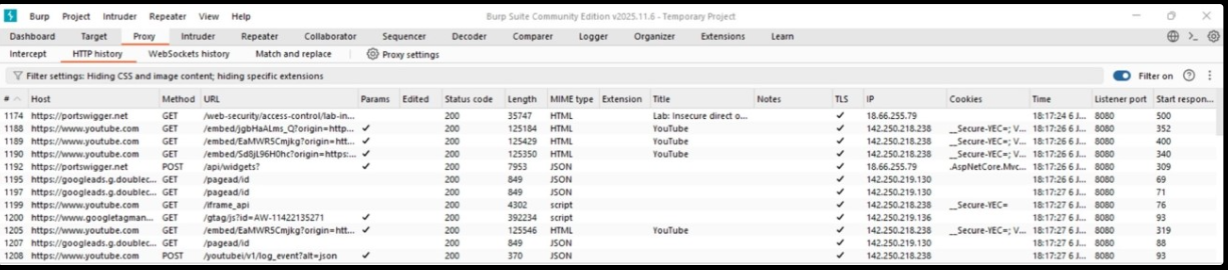
\includegraphics[scale=0.34]{requisicoes}
\end{figure}
\end{frame}



	\begin{frame}[allowframebreaks]{Referências Bibliográficas}
		\begin{thebibliography}{9}

		\bibitem{noauthor_undated-xq}
NTP.br. \url{https://ntp.br/conteudo/ntp/}. Acessado em: 6 de agosto de 2026.

\bibitem{Cisco_System_Inc2022-gp}
Cisco System, Inc. (2022). Identificar e Solucionar Problemas do Network Time Protocol (NTP). 26 de setembro de 2022.

\bibitem{ibm}
IBM. (2025). Tivoli Application Dependency Discovery Manager. \url{https://www.ibm.com/docs/pt-br/taddm/7.3.0?topic=problems-synchronization-server}. Acessado em: 6 de agosto de 2026.

\bibitem{cisco}
Cisco. (2025). Use as práticas recomendadas para o Network Time Protocol. \url{https://www.cisco.com/c/pt_br/support/docs/availability/high-availability/19643-ntpm.html}. Acessado em: 6 de agosto de 2026.

\bibitem{suse}
SUSE. (2026). Sincronizando o horário por meio de NTP/NTS. \url{https://documentation.suse.com/pt-br/sle-micro/6.1/html/Micro-ntp-time-synchronization/index.html}. Acessado em: 6 de agosto de 2026.

\bibitem{Moreiras2021}
Moreiras, Antonio Marcos. (2021). NTP e NTS de Forma Correta e Segura, Sincronismo de Tempo na Internet. Nic.br. \url{https://bibliotecadigital.acervo.nic.br/server/api/core/bitstreams/129d1169-25b5-49ce-b015-28ffadc440da/content}. Acessado em: 6 de agosto de 2026.
\end{thebibliography}
	\end{frame}	
	
\end{document}
